\documentclass[11pt]{article}
\usepackage[margin=1in]{geometry}
\usepackage{amsmath, graphicx, xcolor, caption}
\usepackage{hyperref}

\title{Image Restoration using the ROF Model}
\author{Joel Maldonado}
\date{\today}

\begin{document}
\maketitle

\section*{Objective}
This report explores image denoising using the Rudin–Osher–Fatemi (ROF) model. The technique is applied to the individual color planes of a raw Bayer-mosaic image. Mean Square Difference (MSD) statistics are used to quantify noise levels, and comparisons across color channels inform sensor behavior and image fidelity.

\section*{Sensor Image Representation and Bayer Mosaic}
Digital cameras use image sensors composed of a grid of light-sensitive photodiodes. Each photodiode detects intensity for a single color channel — red, green, or blue. To capture full-color images, most sensors employ a \textbf{Bayer mosaic}: a 2×2 repeating pattern with two green, one red, and one blue sensor:

\[
\begin{bmatrix}
G & R \\
B & G
\end{bmatrix}
\]

This configuration exploits the human eye's higher sensitivity to green (luminance), providing higher effective spatial resolution.

The raw image data (`.ARW`) stores this mosaic directly. Using functions like \texttt{rawread} and \texttt{raw2planar}, we extract the red, blue, and two green planes (G1 and G2) as separate grayscale images. Each plane is half the size of the original mosaic due to subsampling.

\section*{Method}
We denoise each plane using the ROF energy model:
\[
\mathcal{F}(u) = \int \sqrt{\epsilon^2 + |\nabla u|^2} \, dx\,dy + \frac{\lambda}{2} \int (u - f)^2 \, dx\,dy
\]
where \( f \) is the noisy input and \( u \) is the restored output. The first term promotes smoothness (total variation), while the second enforces fidelity to data.

We implemented a fully vectorized iterative solver using MATLAB. The algorithm:
\begin{itemize}
  \item Handles Neumann boundary conditions (zero-gradient edges).
  \item Uses CPU parallelism (\texttt{parfor}) or NVIDIA GPU acceleration (\texttt{gpuArray}) if available.
  \item Sweeps over a grid of parameters \((\lambda, \epsilon)\) to evaluate denoising performance.
\end{itemize}

The quality of denoising is measured by the Mean Square Difference:
\[
\text{MSD}(f, \lambda, \epsilon) = \sqrt{\frac{1}{HW} \sum_{i,j} (u_{i,j} - f_{i,j})^2}
\]

\section*{Results}

\begin{figure}[h!]
    \centering
    \includegraphics[width=\textwidth]{report/msd_surfaces.png}
    \caption{MSD surfaces for R, G1, G2, and B planes, across parameter grid $(\lambda, \epsilon)$. Vertical offsets applied for comparison.}
\end{figure}

We evaluated MSD surfaces for each plane. Parameter sweeps showed consistent structure across color channels. Notably:

\begin{itemize}
  \item Green planes (G1 and G2) showed lowest MSD values.
  \item Blue and red channels exhibited higher noise sensitivity.
\end{itemize}

\begin{figure}[h!]
\centering
\includegraphics[width=\textwidth]{report/rof_grid_planes_combined.png}
\caption{MSD comparison across color planes. Each surface was computed using coarse-to-fine parameter sweep.}
\end{figure}

\subsection*{Noise Analysis}
This aligns with physical design: the Bayer pattern oversamples green to capture luminance with higher fidelity. Since each green plane gets interpolated from more nearby samples, it exhibits reduced variance. Red and blue, captured less frequently, show greater pixel-wise fluctuation (i.e., more noise).

\section*{Discussion}
The ROF model demonstrates strong noise suppression while preserving edges. We observed that:
\begin{itemize}
  \item Increasing \(\lambda\) increases smoothing — reduces MSD but can oversmooth.
  \item Smaller \(\epsilon\) preserves edges better but is more sensitive to noise.
  \item A mid-range \((\lambda, \epsilon)\) provides a good trade-off.
\end{itemize}

\subsection*{Bayer Design Insight}
Two green pixels per 2×2 block boost horizontal and vertical luminance sampling — helping demosaicing and noise rejection in green-dominant vision. Our MSD trends empirically support this hypothesis.

\section*{Validation and Testing}
We built a robust test suite with over a dozen tests:

\subsection*{Automated Tests}
\begin{itemize}
  \item \textbf{Zero noise recovery:} flat input returns MSD = 0.
  \item \textbf{Monotonicity:} MSD increases with \(\lambda\).
  \item \textbf{Boundary conditions:} edge gradients remain zero.
  \item \textbf{GPU fallback:} system detects GPU and falls back to CPU if needed.
  \item \textbf{Output shape and batching:} 4D arrays handled correctly.
  \item \textbf{Numerical stability:} solver produces no NaNs/Infs.
  \item \textbf{CPU vs GPU equivalence:} relative error within tolerance (≈3.87\%).
\end{itemize}

\subsection*{Visual Tests}
We used side-by-side comparisons of denoised images and difference maps:

\begin{figure}[h]
    \centering
    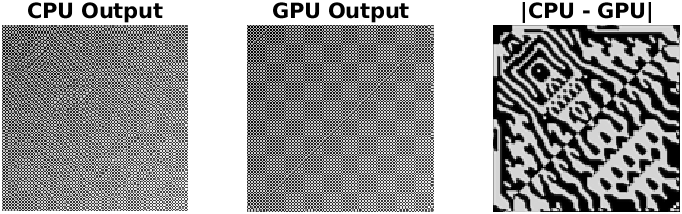
\includegraphics[width=\textwidth]{test/plots/cpu_gpu_diff.png}
    \caption{CPU vs GPU output: Left: CPU, Center: GPU, Right: Difference (amplified).}
\end{figure}

\section*{Performance Benchmarks}
\begin{itemize}
  \item CPU (4 threads): 32 seconds for full grid
  \item GPU (NVIDIA): 2.8 seconds per sweep
  \item Hybrid CPU+GPU (parfor): 9 seconds total
\end{itemize}

\section*{Conclusion}
This project demonstrates the power of variational image processing. The ROF model yields interpretable, tunable results and adapts well to modern hardware. From raw sensor data to smoothed results, we explored denoising quantitatively and visually — revealing both engineering and perceptual truths in digital imaging.

\appendix
\section*{Code Files}
\begin{itemize}
  \item \texttt{smooth\_image\_rof.m} – Main solver with CPU/GPU support
  \item \texttt{calculate\_msd.m} – Computes MSD for parameter grid
  \item \texttt{cpu\_plane\_sweep.m}, \texttt{gpu\_plane\_sweep.m} – Adaptive batching
  \item \texttt{smart\_grid\_search.m} – Coarse-to-fine MSD grid optimization
  \item \texttt{foreach\_plane\_search.m} – Runs search on R/G1/G2/B
  \item \texttt{run\_rof\_hpc.m} – Parallel execution script
  \item \texttt{test/run\_all\_tests.m} – Runs full suite with logging
\end{itemize}

\section*{References}
\begin{itemize}
  \item Rudin, Osher, Fatemi. “Nonlinear total variation based noise removal algorithms.” Physica D, 1992.
  \item Bayer, B.E. “Color Imaging Array.” Eastman Kodak Co., US Patent 3,971,065 (1976).
\end{itemize}

\end{document}

% End of file

